% Revised 28 September 2026 following the annotated PDF comments.
% Numerical sources: publication_tables_2026_09_24 and size strata of 28 September.
% Core counts independently checked against the public-release per_ligand_long
% records; see figure-data/core-recovery-audit.csv and core-recovery-counts.csv.
\section{Results}
\label{sec:results}
% Figures transferred from the working Results; sources are in results-data/.
\newcommand{\diversityfigure}{%
\begin{figure}[htbp]
\centering
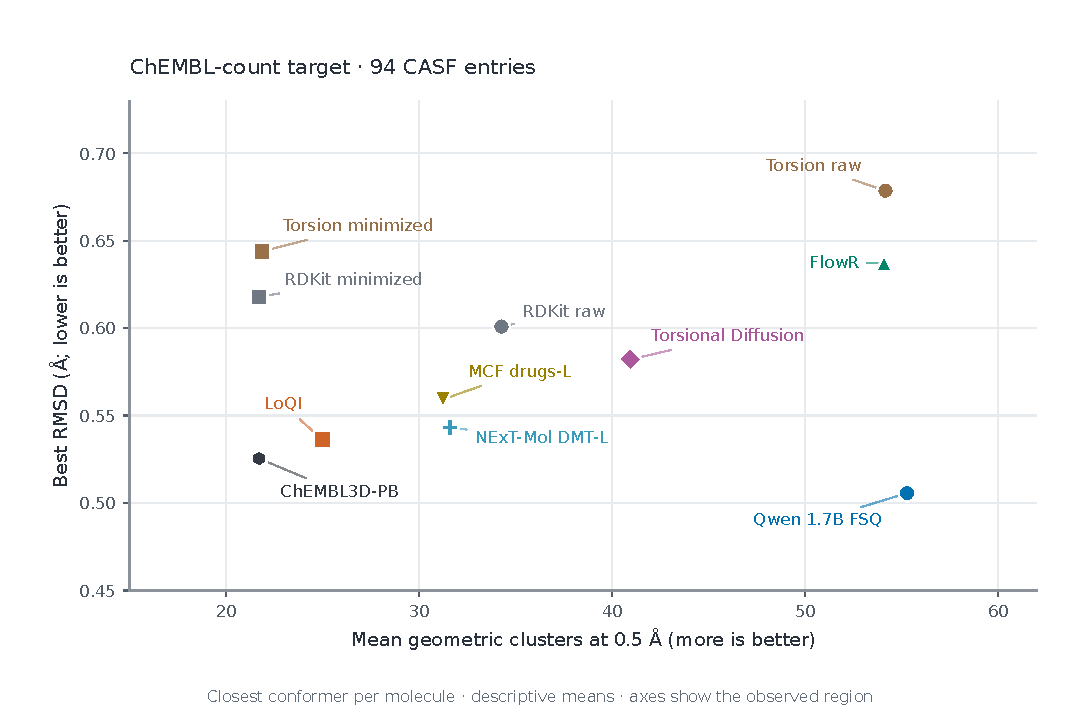
\includegraphics[width=\linewidth]{figures/figure-2-diversity-recovery.pdf}
\caption{Geometric diversity and experimental recovery at the ChEMBL-count target. Each point represents one evaluated pipeline or the stored ChEMBL3D-PB ensemble. Clustering uses a 1.0 \AA{} radius, whereas recovery requires at least one retained conformer at RMSD $\leq$ 0.75 \AA{}. Cluster counts are averaged over defined measurements; recovery uses all 94 entries, including failures. Retained ensemble sizes differ despite matched candidate targets. These are descriptive method summaries, not a causal analysis of diversity.}
\label{fig:diversity-recovery}
\end{figure}}

\newcommand{\recoveryfigure}{%
\begin{figure}[htbp]
\centering
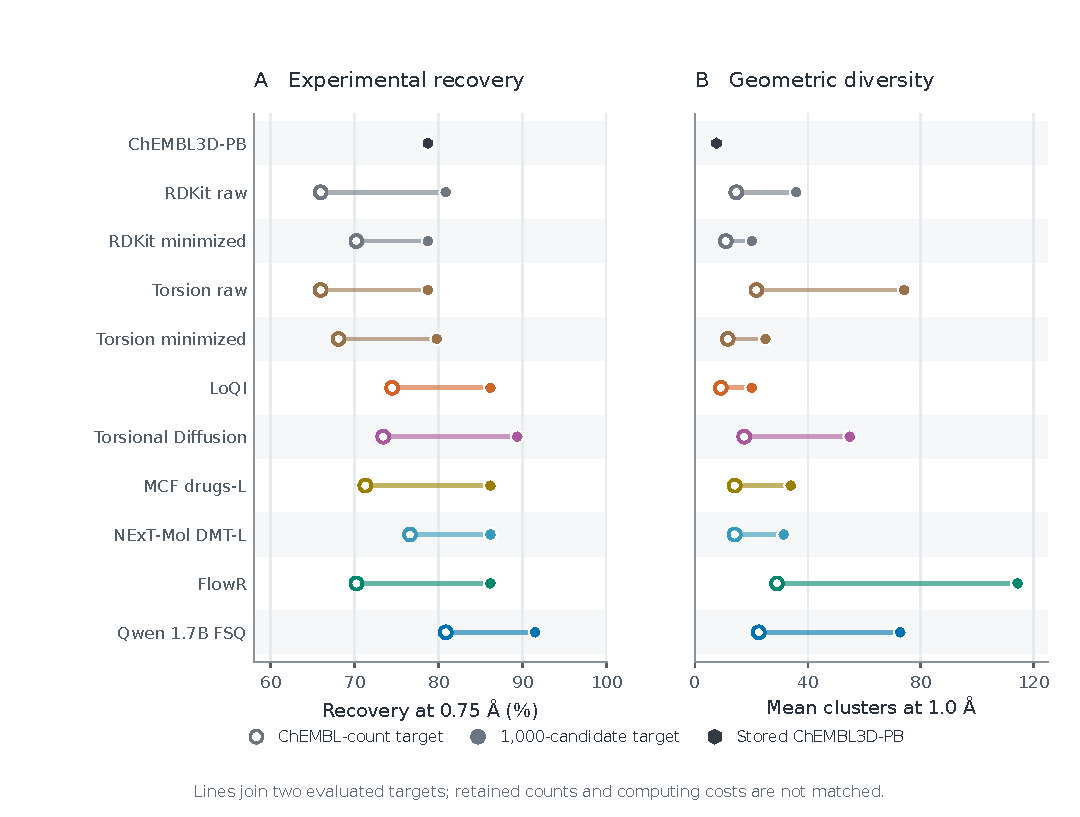
\includegraphics[width=\linewidth]{figures/figure-3-sampling-budget.pdf}
\caption{Recovery and diversity at the two candidate targets. Open circles denote the ChEMBL-count target and filled circles the 1,000-candidate target. Each row follows the same method between the two targets. The stored ChEMBL3D-PB ensemble is shown once as a hexagon. Recovery uses all 94 CASF entries; cluster means use defined measurements. Lines connect observed endpoints and do not represent random-subsampling curves or intermediate measurements. Targets precede PoseBusters filtering; retained counts are given in Table~\ref{tab:recovery}.}
\label{fig:recovery}
\end{figure}}

\newcommand{\sizefigure}{%
\begin{figure}[htbp]
\centering
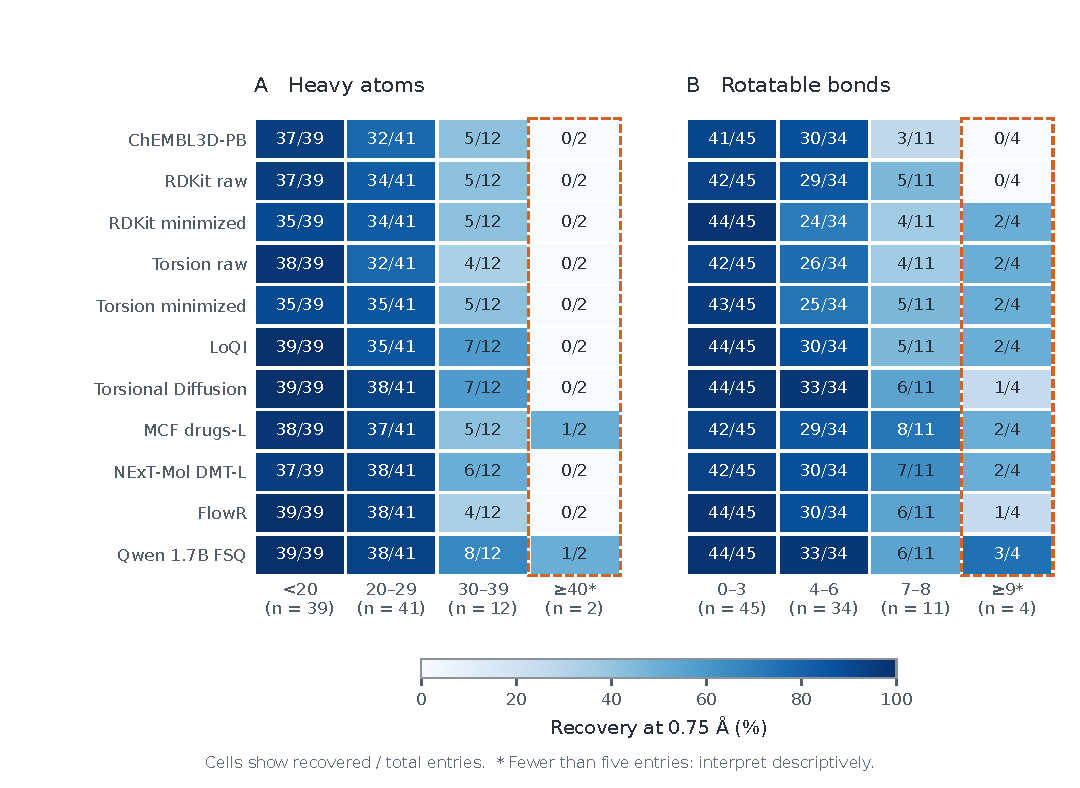
\includegraphics[width=\linewidth]{figures/figure-4-size-flexibility.pdf}
\caption{Recovery by molecular size and flexibility. Generated methods use the 1,000-candidate target; ChEMBL3D-PB uses its stored ensemble. Every cell gives recovered/total CASF entries, with the color indicating the corresponding percentage. Dashed outlines mark groups with fewer than five entries. Heavy-atom and rotatable-bond groups are analyzed separately and do not isolate independent effects of size and flexibility. Sparse groups cannot establish stable method rankings.}
\label{fig:size}
\end{figure}}

\newcommand{\drugfigure}{%
\begin{figure}[htbp]
\centering
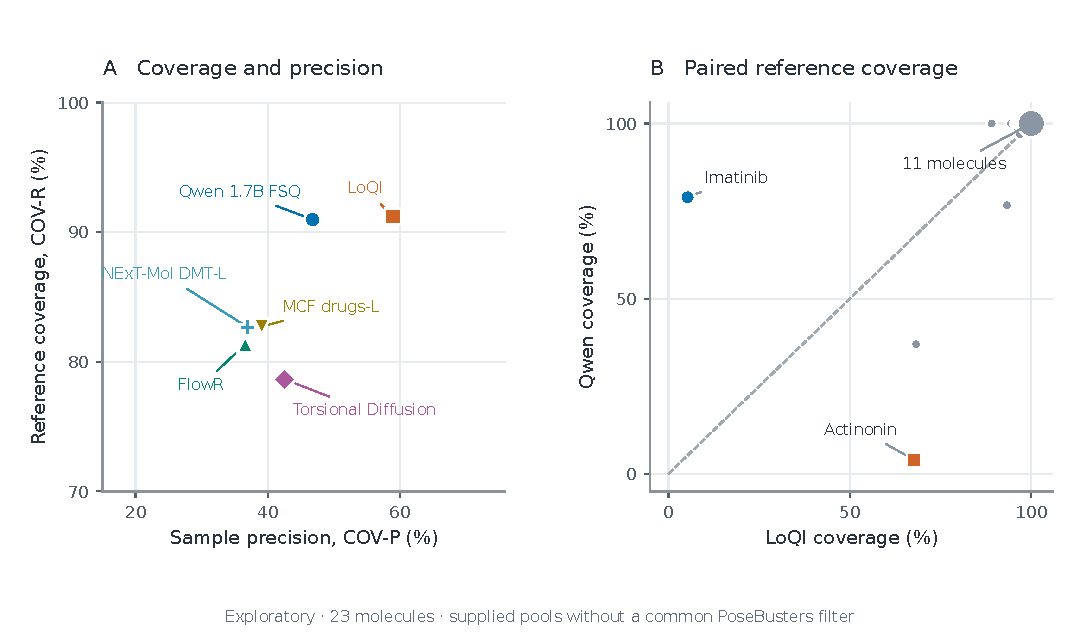
\includegraphics[width=\linewidth]{figures/figure-5-multiple-references.pdf}
\caption{Coverage of multiple bound references and precision relative to those observations. (A) Molecule-averaged COV-R and COV-P for six learned generators, using the existing strict RMSD $<$ 0.75 \AA{} criterion. Axes are restricted to the observed range for readability. (B) Paired reference coverage for Qwen and LoQI across all 23 molecules; the diagonal denotes equal coverage. Coincident points are grouped and labeled, including 11 molecules with complete coverage by both methods. Imatinib and actinonin are the examples retained from the earlier draft. These are descriptive supplied-pool results with differing RMSD-failure conventions, not a comparison after common validity filtering. No uncertainty intervals are shown; paired uncertainty is documented in the archived findings.}
\label{fig:druglike}
\end{figure}}


\subsection{Recovery depended on the sampling allowance}

We compared generators on the core cohort of 94 ligands by counting a ligand
as recovered when at least one conformer passed PoseBusters and lay within
0.75~\AA{} of its experimental geometry. Table~\ref{tab:recovery} presents
two sampling conditions: a candidate target equal to the stored ChEMBL3D
count for each mapped stereoisomer and a fixed target of 1,000 candidates
per ligand. The first tests recovery at an allowance tied to the available
comparison ensemble; the second tests recovery with more extensive sampling.
Both targets apply before filtering, and missing outputs count as failures
in the full denominator of 94 ligands. ChEMBL3D-PB provides the same stored
comparison ensemble for both tiers.
% AUTHOR: document representative-checkpoint selection in Methods; the main
% Qwen model was not the highest-scoring Qwen on every endpoint.

At the ChEMBL-count target, the pretrained Qwen 1.7B FSQ model recovered
76 of 94 ligands (80.9\%), compared with 74 (78.7\%) for ChEMBL3D-PB,
70 (74.5\%) for LoQI, and 69 (73.4\%) for Torsional Diffusion.
Qwen retained a mean of 78.3 conformers per ligand, close to the 81.2 in
the stored ChEMBL3D-PB ensembles. Its paired advantage over ChEMBL3D-PB
was two ligands, or 2.1 percentage points (95\% confidence interval,
$-4.3$ to 8.5), leaving the ordering between them unresolved at this
sampling target.

% Values transferred without recalculation from results-data/results-working.md.
\begin{table}[p]
\centering
\footnotesize
\setlength{\tabcolsep}{4pt}
\renewcommand{\arraystretch}{1.15}
\caption{Recovery and geometric diversity at the two candidate targets on the 94-entry core panel.}
\label{tab:recovery}
\par\smallskip
\textbf{A. Recovery at the two candidate targets}
\par\smallskip
\begin{tabular}{@{}lrrrrrr@{}}
\toprule
Method & \shortstack{ChEMBL-count\\Hit (\%)} & \shortstack{ChEMBL-count\\retained $N$} & \shortstack{ChEMBL-count\\min. RMSD (\AA{})} & \shortstack{1,000\\Hit (\%)} & \shortstack{1,000\\retained $N$} & \shortstack{1,000\\min. RMSD (\AA{})} \\
\midrule
ChEMBL3D-PB & 78.7 & 81.2 & 0.525 & --- & --- & --- \\
RDKit raw & 66.0 & 81.2 & 0.601 & 80.9 & 999.9 & 0.437 \\
RDKit minimized & 70.2 & 81.2 & 0.618 & 78.7 & 1000.0 & 0.512 \\
Torsion raw & 66.0 & 71.1 & 0.679 & 78.7 & 896.5 & 0.477 \\
Torsion minimized & 68.1 & 81.2 & 0.644 & 79.8 & 1000.0 & 0.535 \\
LoQI & 74.5 & 81.2 & 0.536 & 86.2 & 999.3 & 0.339 \\
Torsional Diffusion & 73.4 & 69.3 & 0.582 & 89.4 & 881.4 & 0.371 \\
MCF drugs-L & 71.3 & 66.1 & 0.559 & 86.2 & 866.8 & 0.366 \\
NExT-Mol DMT-L & 76.6 & 66.4 & 0.543 & 86.2 & 871.9 & 0.386 \\
FlowR & 70.2 & 72.7 & 0.637 & 86.2 & 920.0 & 0.414 \\
Qwen 1.7B FSQ & 80.9 & 78.3 & 0.506 & 91.5 & 972.6 & 0.307 \\
\bottomrule
\end{tabular}
\par\smallskip
\begin{minipage}{\linewidth}
Hit uses the 0.75 \AA{} cutoff and all 94 entries. Retained N uses all 94 entries; minimum RMSD is the mean of per-entry best RMSDs, with the same denominator convention as Table~\ref{tab:count-recovery}. At the 1,000-candidate target, minimum RMSD is defined for 93 entries for MCF and NExT-Mol and all 94 for the other pipelines. ChEMBL3D-PB is shown once because its stored ensemble does not grow. These comparisons do not match retained counts or computational cost.
\end{minipage}
\par\bigskip
\textbf{B. Geometric diversity in the larger ensembles}
\par\smallskip
\begin{tabular}{@{}lrr@{}}
\toprule
Method & \shortstack{Mean retained\\conformers} & \shortstack{Mean clusters\\at 1.0 \AA{}} \\
\midrule
ChEMBL3D-PB & 81.2 & 7.7 \\
RDKit raw & 999.9 & 35.9 \\
RDKit minimized & 1000.0 & 20.2 \\
Torsion raw & 896.5 & 74.2 \\
Torsion minimized & 1000.0 & 25.1 \\
LoQI & 999.3 & 20.2 \\
Torsional Diffusion & 881.4 & 54.9 \\
MCF drugs-L & 866.8 & 34.0 \\
NExT-Mol DMT-L & 871.9 & 31.5 \\
FlowR & 920.0 & 114.4 \\
Qwen 1.7B FSQ & 972.6 & 72.8 \\
\bottomrule
\end{tabular}
\par\smallskip
\begin{minipage}{\linewidth}
Generated methods use the 1,000-candidate target; ChEMBL3D-PB remains the same stored ensemble. Cluster means use defined measurements, as in Table~\ref{tab:diversity}.
\end{minipage}
\end{table}


At the target of 1,000 candidates, Qwen recovered 86 of 94 ligands
(91.5\%), compared with 84 for Torsional Diffusion (89.4\%), 81 for LoQI
(86.2\%), and 76 for RDKit without minimization (80.9\%). Qwen recovered
every ligand recovered by ChEMBL3D-PB and 12 additional ligands, giving
a paired difference of 12.8 percentage points (95\% confidence interval,
6.4--20.2). This comparison used a mean of 972.6 retained Qwen conformers
per ligand, however, against the unchanged ChEMBL3D-PB mean of 81.2.
Showing both tiers makes clear that the larger recovery advantage was
achieved with a substantially larger ensemble (Figure~\ref{fig:recovery}B).

The larger ref cohort showed a reversal in the Qwen--ChEMBL3D-PB ordering
between tiers (Table~S2). At the ChEMBL-count target, Qwen recovered 76.3\%
of entries with a mean of 63.3 retained conformers, compared with 78.7\%
and 66.2 for ChEMBL3D-PB. The paired difference was $-2.4$ percentage points
(95\% confidence interval, $-4.7$ to $-0.1$). At 1,000 candidates, Qwen
recovered 92.5\% of the 1,236 entries, compared with 86.8\% for LoQI and
78.7\% for ChEMBL3D-PB. The paired advantage over LoQI was 5.7 percentage
points (3.8--7.7), while excluding compounds shared with core preserved
the advantage over ChEMBL3D-PB (14.0 points; 11.7--16.4). Overlap between
the two evaluation cohorts therefore did not explain the latter comparison,
although this check does not address overlap with model training data.

Together, these comparisons show why recovery rankings must be interpreted
with the sampling allowance. The ChEMBL-count tier consists of subsets of
the available candidate pools, and filtering can leave different retained
counts for different methods. It therefore measures recovery with fewer
sampled candidates without establishing equal computational cost or a
ranking at exactly equal numbers of valid conformers.

\subsection{Closer structural agreement changed the recovery ranking}

Sampling allowance was not the only condition affecting the comparison.
At the target of 1,000 candidates, requiring a closer structural match
reversed the ordering between Qwen and LoQI (Figure~\ref{fig:recovery}A).
At 0.5~\AA{}, LoQI recovered 83.0\% of core ligands and Qwen recovered
78.7\%; at 0.25~\AA{}, the corresponding values were 55.3\% and 53.2\%.
Qwen's higher recovery at the principal cutoff of 0.75~\AA{} thus did
not imply higher recovery at every structural tolerance.

The improvement in recovery also concerned the closest members of the
sampled ensembles. At the fixed target, Qwen's mean minimum RMSD on core
was 0.307~\AA{}, compared with 0.339~\AA{} for LoQI and 0.525~\AA{}
for the stored ChEMBL3D-PB ensembles (Table~S1). In contrast, the means
of their ensemble median RMSDs were similar at 1.318, 1.305, and
1.326~\AA{}, respectively. The higher recovery therefore did not imply
that a typical Qwen conformer was closer to the experimental target.

\recoveryfigure

\subsection{Geometric diversity did not reproduce the recovery ranking}

To examine whether broader geometric sampling accounted for the recovery
ordering at the target of 1,000 candidates, we compared the number of
conformer clusters at a 1.0~\AA{} RMSD radius. FlowR produced more clusters than Qwen on core (114.4 versus
72.8 per ligand), yet recovered fewer targets (86.2\% versus 91.5\%).
Torsion perturbation likewise produced 74.2 clusters, close to Qwen's
count, but recovered only 78.7\% of targets; LoQI reached 86.2\%
recovery with 20.2 clusters. These contrasting outcomes show why cluster
count alone did not provide the same ranking as recovery of experimental
conformations (Figure~\ref{fig:diversity-recovery}B).

The ref cohort showed the same ordering among FlowR, Qwen, and LoQI,
whose mean cluster counts were 105.4, 63.7, and 24.4, respectively, and
whose recovery rates were 85.5\%, 92.5\%, and 86.8\%. The curves across clustering radii in Figure~\ref{fig:diversity-recovery}A place these comparisons
within a range of geometric resolutions. Because cluster counts depend
on both retained ensemble size and clustering order, they describe the
spread of the sampled structures rather than the number of biologically
accessible states.
% AUTHOR: do not reuse a correlation from the 19-checkpoint panel as if it
% described the smaller selection plotted here.

\diversityfigure

\subsection{Recovery varied with molecular size and flexibility}

At the target of 1,000 candidates, stratifying core by heavy-atom count
revealed differences that were obscured by the overall recovery rates (Table~\ref{tab:size}; Figure~\ref{fig:size}).
Qwen, LoQI, and FlowR each recovered all 39 ligands with fewer than 20 heavy
atoms, but their performance separated among the 12 ligands with 30--39
heavy atoms: recovery was 66.7\% for Qwen, 58.3\% for LoQI, 41.7\% for
ChEMBL3D-PB, and 33.3\% for FlowR. Only two core ligands had at least
40 heavy atoms, limiting what could be concluded about the largest molecules.

% Reproduced by docs/publication_size_analysis_2026_09_28.py.
\begin{table}[htbp]
\centering
\small
\setlength{\tabcolsep}{5pt}
\caption{Size-stratified recovery for selected contrasting methods at the fixed candidate target. Entries are Hit@0.75~\AA{} percentages over all entries in each group; heavy-atom counts come from a common experimental reference. ChEMBL3D-PB uses its stored pool. The small largest-size groups should be interpreted descriptively.}
\label{tab:size}
\begin{tabular}{llrrrrr}
\hline
Cohort & Heavy atoms & Entries & ChEMBL3D-PB & LoQI & FlowR & Qwen \\
\hline
core & $<20$ & 39 & 94.9 & 100.0 & 100.0 & 100.0 \\
core & 20--29 & 41 & 78.0 & 85.4 & 92.7 & 92.7 \\
core & 30--39 & 12 & 41.7 & 58.3 & 33.3 & 66.7 \\
core & $\geq40$ & 2 & 0.0 & 0.0 & 0.0 & 50.0 \\
\hline
ref & $<20$ & 547 & 93.4 & 97.8 & 96.5 & 99.6 \\
ref & 20--29 & 513 & 74.9 & 84.4 & 90.8 & 93.8 \\
ref & 30--39 & 152 & 50.0 & 64.5 & 41.4 & 71.7 \\
ref & $\geq40$ & 24 & 8.3 & 29.2 & 0.0 & 33.3 \\
\hline
\end{tabular}
\end{table}


The larger ref cohort provided more observations in these size groups and
supported the same contrasts. Among its 152 entries with 30--39 heavy atoms,
Qwen recovered 71.7\%, LoQI 64.5\%, ChEMBL3D-PB 50.0\%, and FlowR 41.4\%.
However, recovery remained low among the 24 entries with at least 40 heavy
atoms, of which Qwen and LoQI recovered eight and seven, respectively.
The comparison by molecular size therefore identified differences between
methods without establishing reliable recovery of the largest ligands.

Stratification by flexibility showed a related limitation. Across ref ligands
with 0--3, 4--6, 7--8, and at least 9 rotatable bonds, Qwen recovery fell
from 99.4\% to 94.1\%, 73.1\%, and 33.3\%, while ChEMBL3D-PB recovery
was 94.2\%, 73.6\%, 37.0\%, and 17.6\% in the same groups. The greatest
absolute gain over ChEMBL3D-PB occurred in the group with 7--8 rotatable bonds rather than
among the most flexible ligands. Because size and flexibility are related,
these comparisons identify where performance differs without isolating
either descriptor as its cause.

\sizefigure

\subsection{Multiple experimental references separated coverage from concentration}

We extended the recovery comparison to a separate panel of 23 drug molecules
with 2,450 experimental reference records, allowing us to distinguish coverage
of the observed conformations from the concentration of generated samples
near them. Coverage was evaluated on the supplied pools and validity was
assessed separately; because the evaluations do not yet use common PoseBusters filtering
or the same treatment of failed RMSD calculations, the comparisons remain descriptive
(Methods).
% AUTHOR: harmonize the evaluation before final submission and replace this
% qualification and all affected values together. Do not multiply COV by PB yield.

Qwen and LoQI covered similar fractions of the experimental references,
with mean COV-R values of 91.0\% and 91.2\%, respectively
(Table~\ref{tab:druglike}). Their paired difference of $-0.25$ percentage
points had a wide 95\% confidence interval ($-9.1$ to 8.7), leaving the
recall ordering unresolved rather than establishing equivalence. In contrast,
LoQI had higher precision relative to the observed references: COV-P was 59.0\%, compared
with 46.8\% for Qwen, giving a paired difference between Qwen and LoQI of
$-12.2$ points ($-19.8$ to $-4.7$). Similar reference coverage thus
coincided with a greater fraction of LoQI's generated samples lying near
an observed conformation (Figure~\ref{fig:druglike}).

% Coverage means and supplied counts: figure-data/drug_molecule_metrics.csv.
% PB: pooled pass fraction in corrected druglike_summary.csv; assessed separately.
\begin{table}[htbp]
\centering
\small
\caption{Exploratory multi-reference results for 23 druglike molecules. Mean $N$ is the supplied conformer count per molecule before a common validity filter. COV-R and COV-P are molecule-averaged coverage percentages at a strict 0.75~\AA{} cutoff. PB is the separately measured, pooled PoseBusters pass percentage.}
\label{tab:druglike}
\begin{tabular}{lrrrr}
\hline
Method & Mean $N$ & COV-R (\%) & COV-P (\%) & PB (\%) \\
\hline
LoQI & 1000.0 & 91.2 & 59.0 & 90.9 \\
Torsional Diffusion & 1000.0 & 78.6 & 42.6 & 83.4 \\
MCF drugs-L & 1000.0 & 82.7 & 39.1 & 63.7 \\
NExT-Mol DMT-L & 1000.0 & 82.7 & 36.9 & 62.2 \\
FlowR & 961.7 & 81.3 & 36.6 & 78.5 \\
Qwen 1.7B FSQ & 999.2 & 91.0 & 46.8 & 83.7 \\
\hline
\end{tabular}
\par\smallskip
\begin{minipage}{\linewidth}
\footnotesize Coverage does not use a common PB filter, and imported evaluations
handle failed RMSD calculations differently. The coverage columns therefore
do not measure the common validity criterion used in Table~\ref{tab:recovery}.
Matching-distance summaries are provided in Table~S4.
\end{minipage}
\end{table}


The similar mean recall also concealed contrasting outcomes for individual molecules.
Qwen covered 78.9\% of the 57 imatinib references, compared with 5.3\%
for LoQI, whereas the comparison reversed for the 99 actinonin references
(4.0\% versus 67.7\%). Such differences show why average coverage alone
cannot describe performance on individual molecules. They also need to be
interpreted relative to the available observations: the reference collection
is incomplete, its records need not represent distinct conformational states,
and low precision does not establish that unmatched conformers are
physically inaccessible.
% AUTHOR: add inspected structures for imatinib and actinonin if space permits;
% do not assign a ring, torsion, strain, or binding-interaction mechanism without
% examining the conformers.

\drugfigure
